\documentclass{report}

\usepackage{float}
\usepackage{tikz}
\usepackage{listings}

\usetikzlibrary{shapes,arrows}

\title{Main documentation}

% Define block styles

\tikzstyle{block} = [rectangle, draw, text centered, rounded corners,
    text width=5em, minimum height=4em]
\tikzstyle{arrow} = [draw, -latex]

\lstdefinestyle{mainVHDL}
{
    language   = VHDL,
    frame      = single,
    breaklines = true,
    postbreak  = \mbox{\textcolor{red}{$\hookrightarrow$}\space},
    numbers    = left,
    stepnumber = 1,
    tabsize    = 4,
    captionpos = b,
    columns    = fixed
}

\newtheorem{definition}{Definition}[section]

\begin{document}

%%%%%%%%%%%%%%%%%%%%%%%%%%%%%%%%%%%%%%%%%%%%%%%%%%%%%%%%%%%%%%%%%%%%%%%%%%%%%%%%

\chapter {Background - asynchronous circuits}

There are 3 design phases in the construction of an asynchronous circuit:

\begin{itemize}
    \item Channel model specification - defines the communication channels
    between processes
    \item Handshaking protocol specification - defines the signal transitions on
    each communication channel (2-phase or 4-phase)
    \item Data encoding protocol specification - defines the data and
    handshaking assignments to wires (dual rail or bundled data)
\end{itemize}

%%%%%%%%%%%%%%%%%%%%%%%%%%%%%%%%%%%%%%%%%%%%%%%%%%%%%%%%%%%%%%%%%%%%%%%%%%%%%%%%

\section {Channel model specification}

\subsection {Definitions}

A channel exists between 2 processes. Each process connects to zero or more
channels via ports.

The channel specification is orthogonal to the handshaking specification and
the data encoding protocols used.

%%%%%%%%%%%%%%%%%%%%%%%%%%%%%%%%%%%%%%%%%%%%%%%%%%%%%%%%%%%%%%%%%%%%%%%%%%%%%%%%

\subsection {Specification}

\subsubsection {Representation}

The channel model specification can be defined in VHDL and with the aid of
channel model diagrams, as shown in Figure \ref{fig:passive-active-channels}.
Note that the arrow should point to from the process initiating the
communication.

\begin {figure}[H]
\centering
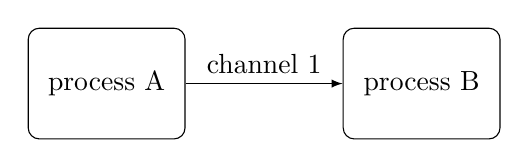
\begin{tikzpicture}[auto]

    % Place nodes
    \node [block] (processA) {process A};
    \node [block, right of=processA, node distance=4cm] (processB) {process B};

    % Draw edges
    \path [arrow]
    (processA)
    -- node [midway,above ] { channel 1}
    (processB);

\end{tikzpicture}
\caption {Channel between process A (producer) and process B (consumer).}
\label {fig:passive-active-channels}
\end {figure}

Given 2 processes, producer and consumer, and a channel between them, the VHDL
channel description is shown in Listing \ref{lst:active-passive-channel}.

\begin{lstlisting} [caption = {Channel between producer and consumer processes},
                    style   = mainVHDL,
                    label   = {lst:active-passive-channel}]
entity async_block is
end entity async_block;

architecture channel_spec of async_block is
    -- Channel
    signal ChannelProdToCons : channel := init_channel;

    -- Data units
    signal producedData : std_logic_vector(2 downto 0);
    signal consumedData : std_logic_vector(2 downto 0);
begin
    producer : process
    begin
        producedData <= selection(8, 3); -- 3 bits, 8 possibilities

        wait for delay(5, 10); -- Random delay between 5-10 units

        send(ChannelProdToCons, producedData);
    end process producer;

    consumer : process
    begin
        receive(ChannelProdToCons, consumedData);

        wait for delay(2, 5); -- Consume data
    end process consumer;
end architecture channel_spec;
\end{lstlisting}

Here the data and control signals are sent over the channel. The
\lstinline{producedData} is copied on the channel on the producer side. On the
consumer side the data from the channel is copied on the local
\lstinline{consumedData} signals.

Ideally, the consumers and producers should be defined as separate components,
as shown in Listing \ref{lst:independent-producer-consumer}.

\begin{lstlisting} [caption = {Consumer and producer are independent},
                    style   = mainVHDL,
                    label   = {lst:independent-producer-consumer}]
-- producer.vhd

entity producer is
    port(channelToConsumer : inout channel := init_channel);
end entity producer;

architecture channel_spec of producer is
    signal producedData : std_logic_vector(2 downto 0);
begin
    main : process
    begin
        producedData <= selection(8, 3);

        wait for delay(5, 10);

        send(channelToConsumer, producedData);
    end process main;
end architecture channel_spec;

-- consumer.vhd

entity consumer is
    port(channelFromProducer : inout channel := init_channel);
end entity consumer;

architecture channel_spec of consumer is
    signal consumedData : std_logic_vector(2 downto 0);
begin
    main : process
    begin
        receive(channelFromProducer, consumedData);

        wait for delay(2, 5);
    end process main;
end architecture channel_spec;
\end{lstlisting}

%%%%%%%%%%%%%%%%%%%%%%%%%%%%%%%%%%%%%%%%%%%%%%%%%%%%%%%%%%%%%%%%%%%%%%%%%%%%%%%%

\subsubsection{Deadlocks}

A port can be either active or passive.

The process with the active port initiates the communication (handshaking) while
the process with the passive port waits for an initiation.

For valid communication (without deadlocks) to occur, a channel shall be
connected to a passive port on one end and an active port on the other end.

Deadlocks may occur when processes handle multiple channels. While waiting to
receive data on one channel, the other process is trying to send data on another
channel, as shown in Listing \ref{lst:deadlock-example}.

\begin {figure}[H]
\centering
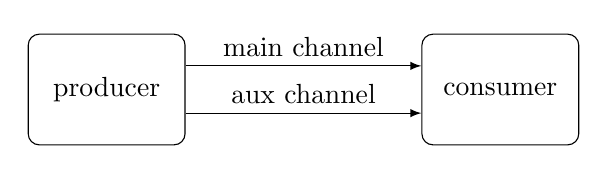
\begin{tikzpicture}[auto]

    % Place nodes
    \node [block] (processA) {producer};
    \node [block, right of=processA, node distance=5cm] (processB) {consumer};

    % Draw edges
    \path [arrow]
    ([yshift = 0.3cm] processA.east)
    -- node [midway,above] { main channel }
    ([yshift = 0.3cm] processB.west);

    \path [arrow]
    ([yshift = -0.3cm] processA.east)
    -- node [midway,above] { aux channel}
    ([yshift = -0.3cm] processB.west);

\end{tikzpicture}
\caption {Multiple channels between a consumer and producer.}
\label {fig:multiple-channels}
\end {figure}

\begin{lstlisting} [caption = {Deadlock example},
                    style   = mainVHDL,
                    label   = {lst:deadlock-example}]
producer : process
begin
    wait for delay(5, 10);
    send(mainChannelToConsumer, mainProducedData);

    wait for delay(5, 10);
    send(auxChannelToConsumer, auxProducedData);
end process main;

consumer : process
begin
    receive(auxChannelFromProducer, auxConsumedData); -- Deadlock
    receive(mainChannelFromProducer, mainConsumedData);

    wait for delay(2, 5);
end process main;
\end{lstlisting}

The producer tries to send data on the main channel while the consumer is
waiting for data on the aux channel.

\textbf{Note:} To prevent deadlocks, the consumer has to first probe the
channels to check if they have data on them. Only then the consumer may receive
data on those channels, as shown in Listing \ref{lst:channel-probing}. This is
not required when a single channel is used between the consumer and producer.

\begin{lstlisting} [caption = {Channel probing},
                    style   = mainVHDL,
                    label   = {lst:channel-probing}]
producer : process
begin
    wait for delay(5, 10);
    send(mainChannelToConsumer, mainProducedData);

    wait for delay(5, 10);
    send(auxChannelToConsumer, auxProducedData);
end process main;

consumer : process
begin
    if (probe(auxChannelFromProducer)) then
        receive(auxChannelFromProducer, auxConsumedData);
    elsif (probe(mainChannelFromProducer)) then
        receive(mainChannelFromProducer, mainConsumedData);
    end if;

    wait for delay(2, 5);
end process main;
\end{lstlisting}

\textbf{Note:} The process which probes a channel should, therefore, be
connected to the passive end of that channel.

%%%%%%%%%%%%%%%%%%%%%%%%%%%%%%%%%%%%%%%%%%%%%%%%%%%%%%%%%%%%%%%%%%%%%%%%%%%%%%%%

\section{Sequential communication}

\subsection{Single channel communication}

Given a single channel between a consumer and a producer, a single unit of data
is communicated at a time. The producer creates a data unit and sends it over
the channel as shown in Listing \ref{lst:single-channel-producer}.

\begin{lstlisting} [caption = {Single channel producer},
                    style   = mainVHDL,
                    label   = {lst:single-channel-producer}]
producer : process
begin
    wait for delay(5, 10);

    send(mainChannel, data);
end process producer;
\end{lstlisting}

The consumer  then receives the data unit as shown in Listing
\ref{lst:single-channel-consumer}.

\begin{lstlisting} [caption = {Single channel consumer},
                    style   = mainVHDL,
                    label   = {lst:single-channel-consumer}]
consumer : process
begin
    receive(mainChannel, data);

    wait for delay(5, 10);
end process consumer;

\end{lstlisting}

This is the simplest way to communicate as it only requires a single channel.
This also expands into a small and simple circuit. The performance however,
is sacrificed as no data can be communicated in parallel.

The resulting connections between the processes is simple as a process
communicates with exactly one other process. Also no deadlocks can occur.

\begin{table}[H]
    \centering
    \begin{tabular}{ r c l }
        process interconnect & \rightarrow & simple \\
        data flow            & \rightarrow & simple \\
        performance          & \rightarrow & low \\
        circuit size         & \rightarrow & small \\
        deadlock chance      & \rightarrow & not possible \\
    \end{tabular}
\end{table}

%%%%%%%%%%%%%%%%%%%%%%%%%%%%%%%%%%%%%%%%%%%%%%%%%%%%%%%%%%%%%%%%%%%%%%%%%%%%%%%%

\subsection{Multiple channel sequential communication}

Given multiple channels connected to a consumer or a producer, a single unit of
data is communicated over a single channel at a time.

This type of communication requires a producer to be connected to multiple
consumers and vice versa as shown in Figure
\ref{fig:multi-channel-communication}. The producer can only produce one data
unit at a time.

\begin {figure}[H]
\centering
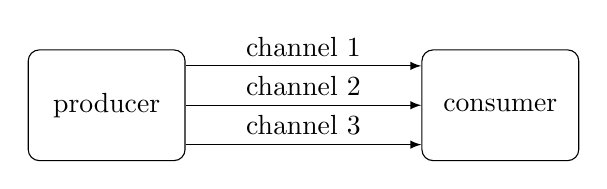
\begin{tikzpicture}[auto]

    % Place nodes
    \node [block] (producer) {producer};
    \node [block, right of=producer, node distance=5cm] (consumer) {consumer};

    % Draw edges
    \path [arrow]
    ([yshift = 0.5cm] producer.east)
    -- node [midway,above] { channel 1 }
    ([yshift = 0.5cm] consumer.west);

    \path [arrow]
    (producer.east)
    -- node [midway,above] { channel 2 }
    (consumer.west);

    \path [arrow]
    ([yshift = -0.5cm] producer.east)
    -- node [midway,above] { channel 3}
    ([yshift = -0.5cm] consumer.west);

\end{tikzpicture}
\caption {Sequential communication over multiple channels.}
\label {fig:multi-channel-communication}
\end {figure}

The resulting connections between processes is complex as a single process
communicates with multiple processes.

\begin{table}[H]
    \centering
    \begin{tabular}{ r c l }
        process interconnect & \rightarrow & complex \\
        data flow            & \rightarrow & simple \\
        performance          & \rightarrow & low \\
        circuit size         & \rightarrow & large \\
        deadlock chance      & \rightarrow & possible unless probing is used \\
    \end{tabular}
\end{table}

\subsubsection{Producer}

The producer creates a data unit and places it on a channel. It then creates
another data unit and places it on another channel (which may be the same as the
previous channel). The producer makes the choice of what data to send over which
channel at any time. No data is communicated in parallel.

As shown in Listing \ref{lst:multi-channel-producer}, the producer sends data
over the second channel, then over the first channel and lastly over the third
channel before restarting the flow.

\begin{lstlisting} [caption = {Multiple channel producer},
                    style   = mainVHDL,
                    label   = {lst:multi-channel-producer}]
consumer : process
begin
    data <= selection(8, 3);
    wait for delay(5, 10);
    send(channel2, data);

    data <= selection(8, 3);
    wait for delay(5, 10);
    send(channel1, data);

    data <= selection(8, 3);
    wait for delay(5, 10);
    send(channel3, data);
end process consumer;

\end{lstlisting}

\subsubsection{Consumer}

The consumer has to check which of the channels has data and then wait to
receive the data from that channel. The consumer makes the choice in which order
to check which channels have data.

The consumer has to also probe the channels to prevent deadlocks as shown in
Listing \ref{lst:multi-channel-consumer-probing}.

\begin{lstlisting} [caption = {Multiple channel consumer with probing},
                    style   = mainVHDL,
                    label   = {lst:multi-channel-consumer-probing}]
consumer : process
begin
    if (probe(channel1)) then
        receive(channel1, data);
    elsif (probe(channel2)) then
        receive(channel2, data);
    elsif (probe(channel3)) then
        receive(channel3, data);
    end if;

    wait for delay(5, 10);
end process consumer;

\end{lstlisting}

If there is a strict protocol which decides which channel to use next and both,
the producer and consumer adhere to it, probing may be skipped as shown in
Listing \ref{lst:multi-channel-consumer-no-probing}.

\begin{lstlisting} [caption = {Multiple channel consumer without probing},
                    style   = mainVHDL,
                    label   = {lst:multi-channel-consumer-no-probing}]
consumer : process
begin
    receive(channel2, data);
    wait for delay(5, 10);

    receive(channel1, data);
    wait for delay(5, 10);

    receive(channel3, data);
    wait for delay(5, 10);
end process consumer;

\end{lstlisting}

%%%%%%%%%%%%%%%%%%%%%%%%%%%%%%%%%%%%%%%%%%%%%%%%%%%%%%%%%%%%%%%%%%%%%%%%%%%%%%%%

\section{Multiple channel parallel communication}

Given multiple channels connected to a producer or a consumer, multiple data
units are communicated over multiple channels at any time.

This is the most complex type of communication as an arbitrary number of data
units can be communicated over an arbitrary number of channels at any time.

\begin{definition}{\textbf{Parallel transaction}
    A set of data units sent over a multiple channels at once.
\end{definition}

Note that the set of data may be sent in parallel to multiple consumers.
Different parts of the parallel transaction may correspond to different
consumers.

\begin{table}[H]
    \centering
    \begin{tabular}{ r c l }
        process interconnect & \rightarrow & complex \\
        data flow            & \rightarrow & complex \\
        performance          & \rightarrow & high \\
        circuit size         & \rightarrow & large \\
        deadlock chance      & \rightarrow & possible unless probing is used \\
    \end{tabular}
\end{table}

\subsection{Producer}

\subsubsection{Strongly indicating parallel communication}

The producer creates N data units and sends them over N channels. After all N
data units have been sent it then creates M data units and sends them over M
channels. N may or may not be the same as M. This allows the producer to
communicate some data on multiple channels at once.

The producer sends all the data units at any time all at once and will only send
more data units once the previous units have been successfully received by the
consumer. It is called strongly indicating as the producer has to wait for all
the sent data to be fully consumed before it can send any further data on
possibly other channels.

\subsubsection{Weakly indicating parallel communication}

The producer may wish to start sending data early if enough but not all data has
been consumed. For instance the producer may send data units on the first 3
channels in parallel. If the data on channels 0 and 1 have been consumed early,
the producer can send more data on channels 0, 1 and possibly other channels but
not channel 2. It is called weakly indicating as only a part of the complex
transaction needs to be completed before the next transaction may start.

\subsection{Consumer}

The consumer may naively just probe each channel and receive data on the
channels with available data. To fully exploit the parallelism advantages, the
consumer should know at any time which producer is sending parallel data on
which channels and them receive that data in parallel. In such case, the
consumer should skip probing and begin receiving data on those channels.

\section{Multistage data flow}

\end{document}
